\chapter{振动和波 光 相对论(选修3-4)}

\section{机械振动}


1.简谐运动

(1)定义:物体在跟位移大小成正比并且总是指向平衡位置的回复力作用下的振动.

(2)平衡位置:物体在振动过程中回复力为零的位置.

(3)回复力

\ding{172}定义:使物体返回到平衡位置的力.

\ding{173}方向:总是指向平衡位置.

\ding{174}来源:属于效果力,可以是某一个力,也可以是几个力的合力或某个力的分力.

(4)简谐运动的两种模型

\ding{172}弹簧振子

\ding{173}单摆

2.简谐运动的公式和图象

(1)简谐运动的表达式

\ding{172}动力学表达式:F=-kx,其中``-''表示回复力与位移的方向相反.

\ding{173}运动学表达式:x=Asin($\omega t+\varphi$) ,其中A代表振幅,$\omega$=2πf表示简谐运动的快慢,($\omega t+\varphi$)代表简谐运动的相位,$\varphi$叫做初相.

(2)简谐运动的图象

\ding{172}从平衡位置开始计时,函数表达式为x=Asin $\omega$t,图象如图甲所示.

\ding{173}从最大位移处开始计时,函数表达式为x=Acos $\omega$t,图象如图乙所示.

\begin{center}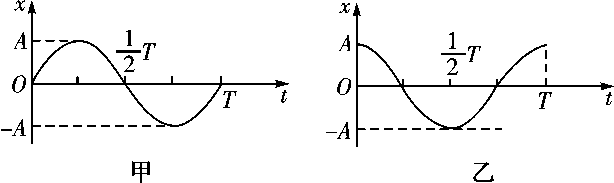
\includegraphics[width=2.79236in,height=0.82986in]{media/image511.png}\end{center}

3.简谐运动的运动规律

(1)对称规律

\ding{172}做简谐运动的物体,在关于平衡位置对称的两点,回复力、位移、加速度具有等大反向的关系.另外,速度的大小、动能具有对称性,速度的方向可能相同或相反.

\ding{173}振动物体来回通过相同的两点间的时间相等,如$t_{BC}=t_{CB}$;振动物体经过关于平衡位置对称的等长的两线段的时间相等,如$t_{BC}=t_{B^\prime C^\prime}$,如图所示.

\begin{center}
\includegraphics[width=1.42431in,height=0.14167in]{media/image512.png}\end{center}

(2)运动的周期性特征

相隔T或nT的两个时刻振动物体处于同一位置且振动状态相同.

4.受迫振动和共振

(1)受迫振动

系统在驱动力作用下的振动.做受迫振动的物体,它做受迫振动的周期(或频率)等于驱动力的周期(或频率),而与物体的固有周期(或频率)无关.

\begin{center}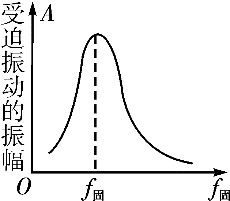
\includegraphics[width=1.04722in,height=0.91528in]{media/image513.png}\end{center}

(2)共振

做受迫振动的物体,它的驱动力的频率与固有频率越接近,其振幅就越大,当二者相等时,振幅达到最大,这就是共振现象.共振曲线如图所示.

\newpage
\subsection{简谐运动的五个特征}

1.动力学特征

F=-kx,``-''表示回复力的方向与位移方向相反,k是比例系数,不一定是弹簧的劲度系数.

2.运动学特征

$a=-\dfrac{k}{m}x$,简谐运动的加速度与物体偏离平衡位置的位移成正比而方向相反,为变加速运动,远离平衡位置时,x、F、a、$E_p$均增大,v、$E_k$均减小,靠近平衡位置时则相反.

3.运动的周期性特征

相隔T或nT的两个时刻振子处于同一位置且振动状态相同.

4.对称性特征

(1)相隔$\dfrac{T}{2}$或$\dfrac{(2n+1)T}{2}$(n为正整数)的两个时刻,振子位置关于平衡位置对称,位移、速度、加速度大小相等,方向相反.

(2)如图所示,振子经过关于平衡位置O对称的两点P、$P^\prime(OP=OP^\prime)$时,速度的大小、动能、势能相等,相对于平衡位置的位移大小相等.

\begin{center}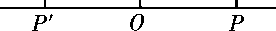
\includegraphics[width=1.25486in,height=0.14167in]{media/image515.png}\end{center}

(3)振子由P到O所用时间等于由O到P'所用时间,即$t_{PO}=t_{OP^\prime}$. 

(4)振子往复过程中通过同一段路程(如OP段)所用时间相等,即$t_{OP}=t_{PO}$.

5.能量特征

振动的能量包括动能$E_k$和势能$E_p$,简谐运动过程中,系统动能与势能相互转化,系统的机械能守恒.

\begin{center}
\includegraphics[width=0.70764in,height=0.12292in]{media/image37.png}\end{center}
\begin{center}
  \textbf{分析简谐运动的技巧}
\end{center}

(1)分析简谐运动中各物理量的变化情况时,一定要以位移为桥梁,位移增大时,振动质点的回复力、加速度、势能均增大,速度、动能均减小;反之,则产生相反的变化.另外,各矢量均在其值为零时改变方向.

(2)分析过程中要特别注意简谐运动的周期性和对称性.

\newpage
\subsection{简谐运动的图象}

1.根据简谐运动图象可获取的信息

(1)振幅A、周期T(或频率f)和初相位$\varphi$(如图所示).

\begin{center}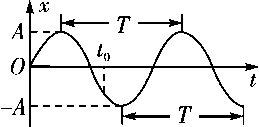
\includegraphics[width=1.17917in,height=0.57569in]{media/image516.png}\end{center}

(2)某时刻振动质点离开平衡位置的位移.

(3)某时刻质点速度的大小和方向:曲线上各点切线的斜率的大小和正负分别表示各时刻质点的速度的大小和速度的方向,速度的方向也可根据下一时刻物体的位移的变化来确定.

(4)某时刻质点的回复力和加速度的方向:回复力总是指向平衡位置,回复力和加速度的方向相同,在图象上总是指向t轴.

(5)某段时间内质点的位移、回复力、加速度、速度、动能和势能的变化情况.

2.利用简谐运动图象理解简谐运动的对称性

\begin{center}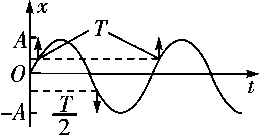
\includegraphics[width=1.17917in,height=0.61319in]{media/image517.png}\end{center}

(1)相隔$\Delta t=n+\dfrac{1}{2}T$
(n=0,1,2,\ldots)的两个时刻,弹簧振子的位置关于平衡位置对称,位移等大反向,速度也等大反向.

(2)相隔$\Delta$t=nT
(n=0,1,2,\ldots)的两个时刻,弹簧振子在同一位置,位移和速度都相同.

\newpage
\subsection{受迫振动和共振}

1.自由振动、受迫振动和共振的比较

\begin{longtable}[]{@{}m{2cm}m{3cm}m{3cm}m{3cm}@{}}
\toprule
&
自由振动
&
受迫振动
&
共振
\tabularnewline
\midrule
\endhead
受力情况 & 仅受回复力 & 受驱动力作用 & 受驱动力作用\tabularnewline
振动周期

或频率
&
由系统本身性质决定,即固有周期$T_0$或固有频率$f_0$
&
由驱动力的周期或频率决定,即$T=T_\text{驱}$或$f=f_\text{驱}$
&
$T_\text{驱}=T_0$或$f=f_\text{驱}=f_0$
\tabularnewline
振动能量 & 振动物体的机械能不变 & 由产生驱动力的物体提供 &
振动物体获得的能量最大\tabularnewline
常见例子 & 弹簧振子或单摆($\theta \leq 5^\circ$) & 机械工作时底座发生的振动 &
共振筛、声音的共鸣等\tabularnewline
\bottomrule
\end{longtable}

\begin{center}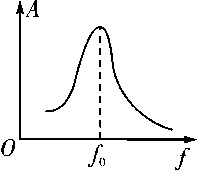
\includegraphics[width=0.89653in,height=0.77361in]{media/image519.png}\end{center}

2.对共振的理解

(1)共振曲线:如图所示,横坐标为驱动力频率$f$,纵坐标为振幅A.它直观地反映了驱动力频率对某振动系统受迫振动振幅的影响,由图可知,$f$与$f_0$越接近,振幅A越大;当$f=f_0$时,振幅A最大.

(2)受迫振动中系统能量的转化:受迫振动系统机械能不守恒,系统与外界时刻进行能量交换.

\begin{center}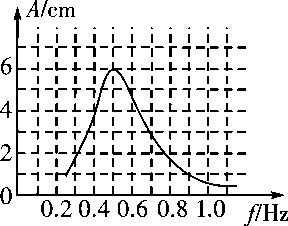
\includegraphics[width=1.31111in,height=1.02847in]{media/image520.png}\end{center}

\begin{center}
\includegraphics[width=0.70764in,height=0.12292in]{media/image13.png}\end{center}

(1)无论发生共振与否,受迫振动的频率都等于驱动力的频率,但只有发生共振现象时振幅才能达到最大.

(2)受迫振动系统中的能量转化不再只有系统内部动能和势能的转化,还有驱动力对系统做正功补偿系统因克服阻力而损失的机械能.

\newpage
\section{机械波}




1.机械波的形成和传播

(1)产生条件

\ding{172}有波源.

\ding{173}有介质,如空气、水、绳子等.

(2)传播特点

\ding{172}传播振动形式、能量和信息.

\ding{173}质点不随波迁移.

\ding{174}介质中各质点振动频率、振幅、起振方向等都与波源相同.

2.机械波的分类

横波和纵波.

3.描述机械波的物理量

(1)波长$\lambda$

在波动中,振动相位总是相同的两个相邻质点间的距离.用``$\lambda$''表示.

(2)频率f

在波动中,介质中各质点的振动频率都是相同的,都等于波源的振动频率.

(3)波速v、波长$\lambda$和频率f、周期T的关系

公式:$v=\dfrac{\lambda}{T}=\lambda f$.

机械波的速度大小由介质决定,与机械波的频率无关.

4.波的图象

\begin{center}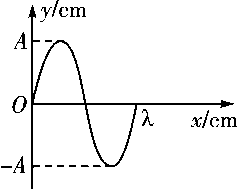
\includegraphics[width=1.07569in,height=0.85833in]{media/image526.png}\end{center}

(1)坐标轴

横轴表示各质点的平衡位置,纵轴表示该时刻各质点的位移.

(2)图象的意义

表示在波的传播方向上,某时刻各质点离开平衡位置的位移.

(3)图象的应用

\ding{172}直接读取振幅A和波长$\lambda$,以及该时刻各质点的位移.

\ding{173}确定某时刻各质点加速度的方向,并能比较其大小.

\ding{174}结合波的传播方向可确定各质点的振动方向或由各质点的振动方向确定波的传播方向.

5.波的干涉和衍射现象 多普勒效应

(1)波的干涉和衍射

\begin{longtable}[]{@{}m{1cm}m{4cm}m{5cm}@{}}
\toprule
& 波的干涉 & 波的衍射\tabularnewline
\midrule
\endhead
条件 & 两列波的频率必须相同,相位差保持不变 &
产生明显衍射的条件:障碍物或孔的尺寸比波长小或相差不多\tabularnewline
现象 & 形成加强区和减弱区相互隔开的稳定的干涉图样 &
波能够绕过障碍物或孔继续向前传播\tabularnewline
\bottomrule
\end{longtable}

(2)多普勒效应

\ding{172}条件:声源和观察者之间有相对运动;

\ding{173}现象:观察者感到频率发生变化;

\ding{174}实质:声源频率不变,观察者接收到的频率变化.
\subsection{对波动图象的理解与应用}

1.波的图象描述的是在波的传播方向上,介质中的各个质点在某一时刻相对各自平衡位置的位移.

2.在波的传播方向上,当两质点平衡位置间的距离为$n\lambda$
(n=1,2,3,\ldots)时,它们的振动步调总相同;当两质点平衡位置间的距离为(2n+1)$\dfrac{\lambda}{2}$
(n=0,1,2,3,\ldots)时,它们的振动步调总相反.

3.波源质点的起振方向决定了它后面的质点的起振方向,各质点的起振方向与波源的起振方向相同.

\begin{center}
\includegraphics[width=0.70764in,height=0.12292in]{media/image37.png}\end{center}
\begin{center}
  \textbf{波的传播方向与质点振动方向的互判方法}
\end{center}

\begin{longtable}[]{@{}m{2cm}m{6cm}m{3cm}@{}}
\toprule
& 内容 & 图象\tabularnewline
\midrule
\endhead
``上下坡''法 &
沿波的传播方向,``上坡''时质点向下振动,``下坡''时质点向上振动 &
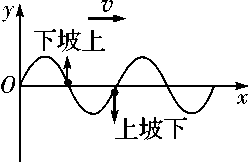
\includegraphics[width=1.13194in,height=0.73611in]{media/image528.png}\tabularnewline
``同侧''法 & 波形图上某点表示传播方向和振动方向的箭头在图线同侧 &
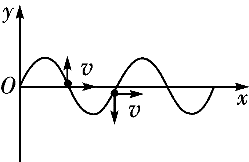
\includegraphics[width=1.13194in,height=0.73611in]{media/image529.png}\tabularnewline
``微平移''法 &
将波形沿传播方向进行微小的平移,再由对应同一x坐标的两波形曲线上的点来判断振动方向
&
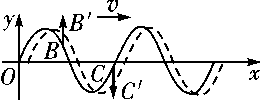
\includegraphics[width=1.18889in,height=0.45278in]{media/image530.png}\tabularnewline
\bottomrule
\end{longtable}

\newpage
\subsection{振动图象和波动图象的综合应用}

振动图象与波动图象的比较

\begin{longtable}[]{@{}m{2cm}m{5cm}m{5cm}@{}}
\toprule
& 振动图象 & 波动图象\tabularnewline
\midrule
\endhead
研究对象 & 一振动质点 & 沿波传播方向所有质点\tabularnewline
研究内容 & 一质点位移随时间变化规律 &
某时刻所有质点的空间分布规律\tabularnewline
图象 &
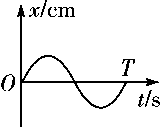
\includegraphics[width=0.72639in,height=0.57569in]{media/image532.png} &
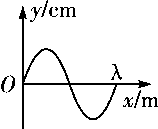
\includegraphics[width=0.71667in,height=0.58472in]{media/image533.png}\tabularnewline
物理意义 & 表示同一质点在各时刻的位移 &
表示某时刻各质点的位移\tabularnewline
\begin{minipage}[t]{0.30\columnwidth}\raggedright
图象信息\strut
\end{minipage} & \begin{minipage}[t]{0.30\columnwidth}\raggedright
(1)质点振动周期

(2)质点振幅

(3)各时刻质点位移

(4)各时刻速度、加速度方向\strut
\end{minipage} & \begin{minipage}[t]{0.30\columnwidth}\raggedright
(1)波长、振幅

(2)任意一质点此刻的位移

(3)任意一质点在该时刻加速度方向

(4)传播方向、振动方向的互判\strut
\end{minipage}\tabularnewline
形象比喻 & 记录着一个人一段时间内活动的录像带 &
记录着许多人某时刻动作、表情的集体照片\tabularnewline
图象变化 & 随时间推移图象延续,但已有形状不变 &
随时间推移,波形沿传播方向平移\tabularnewline
一完整曲线占横坐标距离 & 表示一个周期 & 表示一个波长\tabularnewline
\bottomrule
\end{longtable}

\begin{center}
\includegraphics[width=0.70764in,height=0.12292in]{media/image37.png}\end{center}
\begin{center}
  \textbf{巧解波动图象与振动图象综合类问题}
\end{center}

(1)分清振动图象与波动图象.只要看清横坐标即可,横坐标为x则为波动图象,横坐标为t则为振动图象.

(2)看清横、纵坐标的单位,注意单位前的数量级.

(3)找准波动图象对应的质点.

(4)找准振动图象对应的时刻.


\newpage  
\subsection{波的多解问题}

1.造成波动问题多解的主要因素

(1)周期性

\ding{172}时间周期性:时间间隔$\Delta$t与周期T的关系不明确;

\ding{173}空间周期性:波传播距离$\Delta$x与波长$\lambda$的关系不明确.

(2)双向性

\ding{172}传播方向双向性:波的传播方向不确定;

\ding{173}振动方向双向性:质点振动方向不确定.

(3)波形的隐含性形成多解

在波动问题中,往往只给出完整波形的一部分,或给出几个特殊点,而其余信息均处于隐含状态.这样,波形就有多种情况,形成波动问题的多解性.

2.解决波的多解问题的思路

一般采用从特殊到一般的思维方法,即找出一个周期内满足条件的关系$\Delta$t或$\Delta$x,若此关系为时间,则t=nT+$\Delta$t
(n=0,1,2,\ldots);若此关系为距离,则x=n$\lambda$+$\Delta$x(n=0,1,2,\ldots).

\begin{center}
\includegraphics[width=0.70764in,height=0.12292in]{media/image37.png}\end{center}
\begin{center}
  \textbf{求解波的多解问题的一般步骤}
\end{center}

(1)根据初、末两时刻的波形图确定传播距离与波长的关系通式.

(2)根据题设条件判断是唯一解还是多解.

(3)根据波速公式v=或v==$\lambda$f求波速.


\subsection{波的干涉和衍射 多普勒效应}

1.波的干涉现象中加强点、减弱点的两种判断方法

(1)公式法

某质点的振动是加强还是减弱,取决于该点到两相干波源的距离之差$\Delta$r.

\ding{172}当两波源振动步调一致时

若$\Delta$r=n$\lambda$ (n=0,1,2,\ldots),则振动加强;

若$\Delta r=(2n+1)\dfrac{\lambda}{2}$ (n=0,1,2,\ldots),则振动减弱.

\ding{172}当两波源振动步调相反时

若$\Delta r=(2n+1)\dfrac{\lambda}{2}$ (n=0,1,2,\ldots),则振动加强;

若$\Delta$r=n$\lambda$ (n=0,1,2,\ldots),则振动减弱.

(2)图象法

在某时刻波的干涉的波形图上,波峰与波峰(或波谷与波谷)的交点,一定是加强点,而波峰与波谷的交点一定是减弱点,各加强点或减弱点各自连接而成以两波源为中心向外辐射的连线,形成加强线和减弱线,两种线互相间隔,加强点与减弱点之间各质点的振幅介于加强点与减弱点的振幅之间.

2.多普勒效应

(1)产生条件:波源与观察者之间有相对运动.

(2)现象:两者相互靠近时,感觉波的频率升高;两者相互远离时,感觉波的频率降低.

\newpage
\section{光的折射 全反射}



1.光的折射定律 折射率

(1)折射现象

光从一种介质斜射进入另一种介质时传播方向发生改变的现象,如图所示.

\begin{center}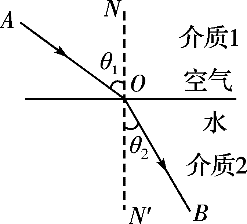
\includegraphics[width=1.12292in,height=1.01875in]{media/image545.png}\end{center}

(2)折射定律

\ding{172}内容:折射光线与入射光线、法线处在同一平面内,折射光线与入射光线分别位于法线的两侧;入射角的正弦与折射角的正弦成正比.

(2)表达式:$\dfrac{\sin\theta_1}{\sin\theta_2}=n_{12}$,式中$n_{12}$是比例常数.

(3)折射率

\ding{172}物理意义:折射率反映介质的光学特征,折射率大,说明光线从真空射入到该介质时偏折大,反之偏折小.

\ding{173}定义式:$n=\dfrac{\sin\theta_1}{\sin\theta_2}$,不能说n与$\sin \theta_1$成正比,与$\sin\theta_2$2成反比.折射率由介质本身的光学性质和光的频率决定.

\ding{174}计算公式:$n=\dfrac{c}{v}$.

2.全反射 光导纤维

(1)光密介质与光疏介质

\begin{longtable}[]{@{}m{1.5cm}m{5cm}m{4cm}@{}}
\toprule
& 
光密介质
&
光疏介质
\tabularnewline
\midrule
\endhead
折射率 & 大 & 小\tabularnewline
光速 & 小 & 大\tabularnewline

相对性&
若n甲\textgreater n乙,则甲是光密介质

若n甲\textless n乙,则甲是光疏介质
&
\tabularnewline
\bottomrule
\end{longtable}

(2)全反射

\ding{172}定义:光从光密介质射入光疏介质,当入射角增大到某一角度时,折射光线将消失,只剩下反射光线的现象.

\ding{173}条件:

a.光从光密介质射向光疏介质.

b.入射角大于或等于临界角.

\ding{174}临界角:折射角等于$90^\circ$时的入射角.若光从光密介质(折射率为n)射向真空或空气时,发生全反射的临界角为C,则$sinC=\dfrac{1}{n}$.介质的折射率越大,发生全反射的临界角越小.

(3)光导纤维

光导纤维的原理是利用光的全反射.

\begin{center}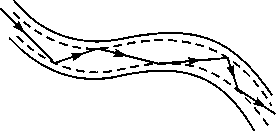
\includegraphics[width=1.25486in,height=0.59444in]{media/image546.png}\end{center}
\subsection{对折射率的理解}

(1)公式$n=\dfrac{\sin\theta_1}{\sin\theta_2}$中,不论光是从真空射入介质,还是从介质射入真空,$\theta_1$总是真空中的光线与法线间的夹角,$\theta_2$总是介质中的光线与法线间的夹角.

(2)折射率由介质本身性质决定,与入射角的大小无关.

(3)折射率与介质的密度没有关系,光密介质不是指密度大的介质.

(4)折射率的大小不仅与介质本身有关,还与光的频率有关.

同一种介质中,频率越大的色光折射率越大,光在介质中的传播速度越小.

(5)同一种色光,在不同介质中虽然波速、波长不同,但频率相同.

2.光路的可逆性

在光的折射现象中,光路是可逆的.如果让光线逆着原来的折射光线射到界面上,光线就会逆着原来的入射光线发生折射.

\begin{center}
\includegraphics[width=0.70764in,height=0.12292in]{media/image13.png}\end{center}
\begin{center}
  \textbf{应用光的折射定律解题的一般思路}
\end{center}

(1)根据入射角、折射角及反射角之间的关系,作出比较完整的光路圈.

(2)充分利用光路图中的几何关系,确定各角之间的联系,根据折射定律求解相关的物理量:折射角、折射率等.

(3)注意在折射现象中,光路是可逆的.

\subsection{光的折射与全反射的综合应用}

1.光密介质和光疏介质是相对而言的.同一种介质,相对于其他不同的介质,可能是光密介质,也可能是光疏介质.

2.如果光线从光疏介质进入光密介质,则无论入射角多大,都不会发生全反射现象.

3.在光的折射和全反射现象中,均遵循光的反射定律,光路均是可逆的.

4.当光射到两种介质的界面上时,往往同时发生光的折射和反射现象,但在全反射现象中,只发生反射,不发生折射.

\begin{center}
\includegraphics[width=0.70764in,height=0.12292in]{media/image13.png}\end{center}
\begin{center}
  \textbf{解决全反射问题的一般方法}
\end{center}

(1)确定光是从光密介质进入光疏介质.

(2)应用$sinC=\dfrac{1}{n}$确定临界角.

(3)根据题设条件,判定光在传播时是否发生全反射.

(4)如发生全反射,画出入射角等于临界角时的临界光路图.

(5)运用几何关系或三角函数关系以及反射定律等进行分析、判断、计算.

\newpage
\subsection{光的色散}

1.光的色散:把复色光分解为单色光的现象叫做光的色散.白光通过棱镜后,被分解为红、橙、黄、绿、蓝、靛和紫七种颜色(如图).

\begin{center}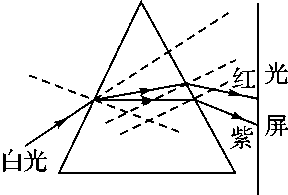
\includegraphics[width=1.31111in,height=0.88681in]{media/image550.png}\end{center}

2.正确理解光的色散

(1)光的颜色由光的频率决定.

(2)各种色光的比较

\begin{longtable}[]{@{}ll@{}}
\toprule
颜色 & 红橙黄绿青蓝紫\tabularnewline
\midrule
\endhead
频率$\nu$ & 低$\rightarrow$高\tabularnewline
同一介质中的折射率 & 小$\rightarrow$大\tabularnewline
同一介质中速度 & 大$\rightarrow$小\tabularnewline
波长 & 大$\rightarrow$小\tabularnewline
临界角 & 大$\rightarrow$小\tabularnewline
通过棱镜的偏折角 & 小$\rightarrow$大\tabularnewline
\bottomrule
\end{longtable}

\newpage
\section{光的波动性 电磁波和相对论}



1.光的干涉

(1)定义:在两列光波叠加的区域,某些区域相互加强,出现亮条纹,某些区域相互减弱,出现暗条纹,且加强区域和减弱区域相互间隔的现象.

(2)条件:两束光的频率相同、相位差恒定.

(3)双缝干涉图样特点:单色光照射时形成明暗相间的等间距的干涉条纹;白光照射时,中央为白色亮条纹,其余为彩色条纹.

2.光的衍射

(1)发生明显衍射的条件

只有当障碍物的尺寸与光的波长相差不多,甚至比光的波长还小的时候,衍射现象才会明显.

(2)衍射条纹的特点

\ding{172}单缝衍射:单色光的衍射图样为中间宽且亮的单色条纹,两侧是明暗相间的条纹,条纹宽度比中央窄且暗;白光的衍射图样为中间宽且亮的白条纹,两侧是渐窄且暗的彩色条纹.

\begin{center}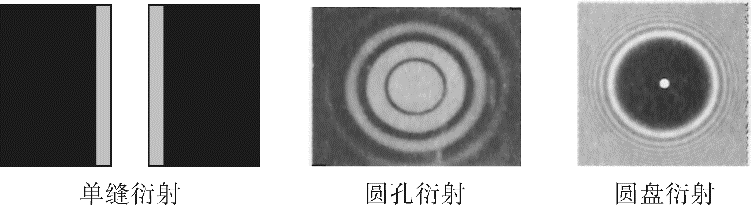
\includegraphics[width=3.41528in,height=0.93403in]{media/image557.png}\end{center}
\ding{173}圆孔衍射:明暗相间的不等距圆环.如图所示.

\ding{174}泊松亮斑(圆盘衍射):当光照到不透明(选填``透明''或``不透明'')的半径很小的小圆盘上时,在圆盘的阴影中心出现亮斑(在阴影外还有不等间距的明暗相间的圆环).如图所示.

3.光的偏振

(1)自然光:包含着在垂直于传播方向上沿一切方向振动的光,而且沿着各个方向振动的光波的强度都相同.

(2)偏振光:在垂直于光的传播方向的平面上,只沿着某个特定的方向振动的光.

(3)偏振光的形成:

\ding{172}让自然光通过偏振片形成偏振光.

\ding{173}让自然光在两种介质的界面发生反射和折射,反射光和折射光可以成为部分偏振光或完全偏振光.

(4)光的偏振现象说明光是一种横波.

4.电磁波的产生

(1)麦克斯韦电磁场理论

变化的磁场产生电场,变化的电场产生磁场.

(2)电磁场

变化的电场和变化的磁场总是相互联系成为一个完整的整体,这就是电磁场.

(3)电磁波

电磁场(电磁能量)由近及远地向周围传播形成电磁波.

\ding{172}电磁波是横波,在空间传播不需要介质;

\ding{173}真空中电磁波的速度为$3.0\times 10^8m/s$;

\ding{174}$v=\lambda f$对电磁波同样适用;

\ding{175}电磁波能产生反射、折射、干涉和衍射等现象.

\newpage
5.电磁波的发射和接收

(1)发射电磁波的条件

\ding{172}要有足够高的振荡频率;

\ding{173}电路必须开放,使振荡电路的电场和磁场分散到尽可能大的空间.

(2)调制有调幅和调频两种方式,解调是调制的逆过程.

(3)电磁波谱

\ding{172}定义:按电磁波的波长从长到短分布是无线电波、红外线、可见光、紫外线、X射线和γ射线,形成电磁波谱;递变规律:直线传播能力增强,衍射能力减弱.

\ding{173}电磁波谱的特性、应用

\begin{longtable}[]{@{}m{1.5cm}m{5cm}m{3.5cm}@{}}
\toprule
电磁波谱 & 特性 & 应用\tabularnewline
\midrule
\endhead
红外线 & 热效应 & 红外线遥感\tabularnewline

紫外线&
化学效应、荧光效应、能杀菌
&
医用消毒、防伪\tabularnewline
X射线 & 贯穿性强 & 检查、医用透视\tabularnewline
$\gamma$射线 & 贯穿本领最强 & 工业探伤、医用治疗\tabularnewline
\bottomrule
\end{longtable}

6.狭义相对论

(1)狭义相对论的两个基本假设

\ding{172}狭义相对性原理:在不同的惯性参考系中,一切物理规律都是相同的.

\ding{173}光速不变原理:真空中的光速在不同的惯性参考系中都是相同的,光速与光源、观测者间的相对运动没有关系.

(2)相对论的质速关系

\ding{172}物体的质量随物体速度的增加而增大,物体以速度v运动时的质量m与静止时的质量$m_0$之间有如下关系:$m=\dfrac{m_0}{\sqrt{1-(\dfrac{v}{c})^2}}$.

\ding{173}物体运动时的质量m总要大于静止时的质量$m_0$.

7.相对论质能关系

用m表示物体的质量,E表示它具有的能量,则爱因斯坦质能方程为:$E=mc^2$.
\newpage
\subsection{光的干涉、衍射和偏振}

1.光的双缝干涉现象

(1)明暗条纹的判断方法

\ding{172}如图所示,光源$S_1$、$S_2$发出的光到屏上P点的路程差$r_2-r_1=k\lambda$
(k=0,1,2,\ldots)时,光屏上出现明条纹.

\begin{center}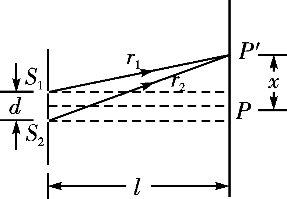
\includegraphics[width=1.30208in,height=0.90556in]{media/image558.png}\end{center}

\ding{173}光的路程差$r_2-r_1=(2k+1)$
(k=0,1,2,\ldots)时,光屏上出现暗条纹.

(2)条纹间距:$\Delta x=\dfrac{L}{d}\lambda$,其中L是双缝到光屏的距离,d是双缝间的距离,$\lambda$是光波的波长.

2.对光的衍射的理解

(1)干涉和衍射是波的特征,波长越长,干涉和衍射现象越明显.在任何情况下都可以发生衍射现象,只是明显与不明显的差别.

(2)衍射现象说明``光沿直线传播''只是一种特殊情况,只有在光的波长比障碍物小得多时,光才可以看做是沿直线传播的.

3.单缝衍射与双缝干涉的比较

\begin{longtable}[]{@{}m{2cm}m{5cm}m{5cm}@{}}
\toprule
&
单缝衍射
&
双缝干涉
\tabularnewline
\midrule
\endhead
条纹宽度
&
条纹宽度不等,中央最宽
&
条纹宽度相等
\tabularnewline
条纹间距 & 各相邻条纹间距不等 & 各相邻条纹等间距\tabularnewline
亮度情况 & 中央条纹最亮,两边变暗 &
条纹清晰,亮度基本相等\tabularnewline
相同点 &\multicolumn{2}{l}{干涉、衍射都是波特有的现象;干涉、衍射都有明暗相间的条纹}
\tabularnewline
\bottomrule
\end{longtable}

4.干涉与衍射的本质

光的干涉条纹和衍射条纹都是光波叠加的结果,从本质上讲,衍射条纹的形成与干涉条纹的形成具有相似的原理.在衍射现象中,可以认为从单缝通过两列或多列频率相同的光波,它们在屏上叠加形成单缝衍射条纹.

5.光的偏振

(1)自然光与偏振光的比较

\begin{longtable}[]{@{}m{2.2cm}m{6cm}m{4cm}@{}}
\toprule
类别 & 自然光(非偏振光) & 偏振光\tabularnewline
\midrule
\endhead
光的来源 & 从普通光源发出的光 & 自然光通过起偏器后的光\tabularnewline
光的振动方向 &
在垂直于光的传播方向的平面内,光振动沿任意方向,且沿各个方向振动的光的强度相同
& 在垂直于光的传播方向的平面内,光振动沿特定方向\tabularnewline
\bottomrule
\end{longtable}

(2)偏振光的应用:加偏振滤光片的照相机镜头、液晶显示器、立体电影、消除车灯眩光等。

\newpage
\subsection{薄膜干涉现象的理解}

1.如图所示,竖直的肥皂薄膜,由于重力的作用,形成上薄下厚的楔形.

\begin{center}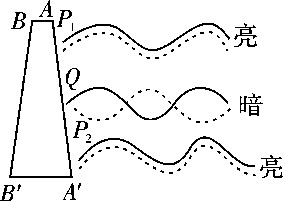
\includegraphics[width=1.28333in,height=0.91528in]{media/image560.png}\end{center}

2.光照射到薄膜上时,在膜的前表面AA$^\prime$和后表面BB$^\prime$分别反射出来,相互叠加,发生干涉.

3.原理分析

(1)单色光

\ding{172}在$P_1$、$P_2$处,两个表面反射回来的两列光波的路程差$\Delta$r等于薄膜中波长的整数倍.

$\Delta$r=n$\lambda$ (n=1,2,3,\ldots),薄膜上出现明条纹.

\ding{173}在Q处,两列反射回来的光波的路程差$\Delta$r等于半波长的奇数倍.$\Delta r=(2n+1)\dfrac{\lambda}{2}$
(n=0,1,2,3,\ldots),薄膜上出现暗条纹.

(2)白光:薄膜上出现水平彩色条纹.

4.薄膜干涉的应用

干涉法检查平面如图所示,两板之间形成一楔形空气膜,用单色光从上向下照射,如果被检平面是平整光滑的,我们会观察到平行且等间距的明暗相间的条纹;若被检平面不平整,则干涉条纹发生弯曲.

\begin{center}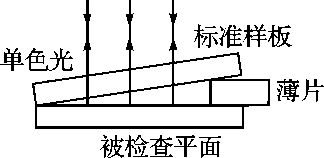
\includegraphics[width=1.47153in,height=0.71667in]{media/image561.png}\end{center}

\newpage
\subsection{电磁场和电磁波}

1.电磁场

如果在空间某区域中有周期性变化的电场,那么这个变化的电场就在它周围空间产生周期性变化的磁场;这个变化的磁场又在它周围空间产生新的周期性变化的电场\ldots\ldots 变化的电场和变化的磁场是相互联系着的,形成不可分割的统一体,这就是电磁场.

2.电磁波的波速、波长与频率的关系:$c=\lambda f$,$\lambda=\dfrac{c}{f}$.

\ding{172}同一种电磁波在不同介质中传播时,频率不变(频率由波源决定),波速、波长发生改变.在介质中的速度都比在真空中速度小.

\ding{173}不同电磁波在同一种介质中传播时,传播速度不同,频率越高波速越小,频率越低波速越大.

3.电磁波与机械波的比较

\begin{longtable}[]{@{}m{2cm}m{5cm}m{5cm}@{}}
\toprule
& 机械波 & 电磁波\tabularnewline
\midrule
\endhead
研究对象 & 研究力学现象 & 研究电磁现象\tabularnewline
周期性变化的物理量 & 位移随时间和空间做周期性变化 &
电场E和磁感应强度B随时间和空间做周期性变化\tabularnewline
传播 & 传播需要介质,波速与介质有关,与频率无关 &
传播无需介质,在真空中波速总是c,在介质中传播时,波速与介质及频率都有关系\tabularnewline
产生 & 由质点(波源)的振动产生 &
由周期性变化的电流(电磁振荡)激发\tabularnewline
纵波还是横波 & 可以是纵波也可以是横波 & 横波\tabularnewline
联系 &\multicolumn{2}{c}{\shortstack{都具有波的一切特性,例如干涉、衍射、反射、折射等性质,\\
它们的波速、波长与频率的关系都是v=$\lambda$f,都能传播能量}}
\tabularnewline
\bottomrule
\end{longtable}

\newpage
\subsection{狭义相对论}

1.对``同时''的相对性的理解:``同时''具有相对性,即在同一个惯性系中不同地点同时发生的两个事件,在另一个惯性系中观察就不一定是同时发生的.

2.对``长度的相对性''的理解:狭义相对论中的长度公式:$l=l_0\sqrt{1-(\dfrac{v}{c})^2}$中,$l_0$是相对于杆静止的观察者测出的杆的长度,而l可认为杆沿杆的长度方向以速度v运动时,静止的观察者测量的长度,或观察者沿杆的长度方向以速度v运动时测出的杆的长度.

3.对``时间间隔的相对性''的理解:时间间隔的相对性公式:$\Delta t=\dfrac{\Delta\tau}{\sqrt{1-(\dfrac{v}{c})^2}}$中$\Delta$τ是相对事件发生地静止的观察者测量同一地点的两个事件发生的时间间隔,而$\Delta$t则是相对于事件发生地以速度v运动的观察者测量同一地点的同样两个事件发生的时间间隔.也就是说:在相对运动的参考系中观测,事件变化过程的时间间隔变大了,这叫做狭义相对论中的时间膨胀.(动钟变慢)

4.对相对论速度变换公式的理解:速度变换公式$u=\dfrac{u^\prime+v}{1+\dfrac{u^\prime v}{c^2}}$.式中u是物体相对静止参考系的速度,v是运动参考系相对静止参考系的速度,$u^\prime$是物体相对运动参考系的速度.($u^\prime$与v同向取正值,反之取负值)


\begin{center}
\includegraphics[width=0.70764in,height=0.12292in]{media/image37.png}\end{center}
\begin{center}
  \textbf{狭义相对论问题的求解技巧}
\end{center}

(1)解决``同时''的相对性问题,可从三个方面入手:

\ding{172}令观察者静止,判断被观察者因相对运动而引起的位置变化.

\ding{173}结合光速不变原理,分析光传播到两个事件所用的时间.

\ding{174}光先传播到的事件先发生,光后传播到的事件后发生.

(2)``动尺缩短''是沿运动方向上的长度比其相对静止时测量的长度要短一些,在垂直于运动方向上的长度没有变化.

(3)``动钟变慢''是两个不同惯性系进行时间比较的结果,也是相对的,即两个惯性系中的观察者都发现对方的钟变慢了.
